% =====================================================================
%  FADO: Fair Oblique Forest -- Online Learning System
%  Publication-quality TikZ system diagram (self-contained, vector only)
%  Compile with:  pdflatex fado_figure.tex
% =====================================================================
\documentclass[tikz,border=6pt]{standalone}
\usepackage{amsmath}
\usepackage{xcolor}
\usetikzlibrary{positioning,fit,calc,backgrounds,arrows.meta,shadows.blur,%
  shapes.misc,shapes.geometric,shapes.symbols,decorations.pathreplacing,matrix}

% =====================================================================
%  COLORS
% =====================================================================
\definecolor{primaryblue}{RGB}{40,90,230}
\definecolor{lightblue}{RGB}{240,246,255}
\definecolor{accorange}{RGB}{245,120,35}
\definecolor{lightorange}{RGB}{255,246,235}
\definecolor{accgreen}{RGB}{55,150,70}
\definecolor{lightgreen}{RGB}{240,250,240}
\definecolor{lightgray}{RGB}{245,245,245}
\definecolor{darktext}{RGB}{45,45,45}

% =====================================================================
%  STYLES
% =====================================================================
\tikzset{
  % --- generic module card (light fill, thin border, very soft shadow) ---
  module/.style={
    rounded corners=4pt, draw, line width=0.6pt, align=center,
    text=darktext, inner sep=5pt, fill=white,
    blur shadow={shadow blur steps=6, shadow xshift=0.3pt,
                 shadow yshift=-0.9pt, shadow opacity=15, shadow blur radius=1.7pt}},
  bluemod/.style  ={module, fill=lightblue!55,   draw=primaryblue!85},
  orangemod/.style={module, fill=lightorange!70, draw=accorange},
  greenmod/.style ={module, fill=lightgreen!75,  draw=accgreen},
  % --- inner sub-panels ---
  sub/.style={rounded corners=2.5pt, draw, line width=0.4pt, align=left,
              inner sep=3pt, font=\scriptsize},
  bluesub/.style  ={sub, fill=white,           draw=primaryblue!35},
  orangesub/.style={sub, fill=white,           draw=accorange!45},
  greensub/.style ={sub, fill=white,           draw=accgreen!35},
  graysub/.style  ={sub, fill=lightgray,       draw=black!18},
  % colour-coded controller phases (cf. reference)
  warnsub/.style  ={sub, fill=yellow!14,  draw=accorange!55, align=left},
  confsub/.style  ={sub, fill=red!7,      draw=red!55,       align=left},
  recovsub/.style ={sub, fill=lightgreen, draw=accgreen!55,  align=left},
  % --- typography ---
  mtitle/.style={font=\bfseries\footnotesize}, % <-- Reduced to \footnotesize
  msub/.style  ={font=\footnotesize\bfseries},
  body/.style  ={font=\scriptsize},
  tiny@/.style ={font=\fontsize{5.0}{5.5}\selectfont},
  % --- arrows : blue solid = data/model flow ; orange dashed = drift/control ---
  dataflow/.style={-{Latex[length=2.6mm,width=2.3mm]}, primaryblue,
                   line width=1.1pt, rounded corners=3pt},
  ctrlflow/.style={-{Latex[length=2.6mm,width=2.3mm]}, accorange,
                   line width=1.1pt, rounded corners=3pt,
                   dash pattern=on 3.5pt off 2pt},
  fairflow/.style={dataflow},
  flowlbl/.style ={font=\fontsize{6}{7}\selectfont\itshape, fill=white,
                   inner sep=1pt, text=darktext},
  % --- dashed grouping containers ---
  groupblue/.style  ={rounded corners=8pt, draw=primaryblue!55, line width=0.8pt,
                      dashed, dash pattern=on 3pt off 2pt},
  grouporange/.style={rounded corners=8pt, draw=accorange!65, line width=0.8pt,
                      dashed, dash pattern=on 3pt off 2pt},
}

% =====================================================================
%  ICONS  (reusable vector pics, ~0.5cm)
% =====================================================================
\tikzset{
  ic/.pic={},
  % brain
  brain/.pic={
    \fill[red!18] (0,0) ellipse (0.24 and 0.19);
    \draw[red!45!black, line width=0.35pt] (-0.13,0.04) .. controls (-0.04,0.13) and (0.04,0.13) .. (0.13,0.03);
    \draw[red!45!black, line width=0.35pt] (-0.14,-0.04) .. controls (0,0.05) .. (0.14,-0.05);
    \draw[red!45!black, line width=0.35pt] (0,0.16)--(0,-0.16);
  },
  % eye
  eye/.pic={
    \draw[darktext, line width=0.5pt] (-0.22,0) .. controls (-0.1,0.15) and (0.1,0.15) .. (0.22,0)
         .. controls (0.1,-0.15) and (-0.1,-0.15) .. (-0.22,0);
    \fill[primaryblue!85] (0,0) circle (0.06);
    \fill[white] (0.02,0.02) circle (0.018);
  },
  % gear
  gear/.pic={
    \foreach \a in {0,45,...,315}{\draw[line width=1.7pt, accgreen!75!black] (\a:0.15)--(\a:0.25);}
    \fill[accgreen!70!black] (0,0) circle (0.16);
    \fill[white] (0,0) circle (0.065);
  },
  % warning triangle
  warning/.pic={
    \fill[accorange] (0,0.24) -- (0.215,-0.15) -- (-0.215,-0.15) -- cycle;
    \draw[accorange!60!black, line width=0.4pt] (0,0.24) -- (0.215,-0.15) -- (-0.215,-0.15) -- cycle;
    \draw[white, line width=0.9pt] (0,0.13)--(0,-0.02);
    \fill[white] (0,-0.08) circle (0.024);
  },
  % balance scale
  scale/.pic={
    \draw[accgreen!70!black, line width=0.7pt] (0,-0.18)--(0,0.2);
    \fill[accgreen!70!black] (0,0.2) circle (0.025);
    \draw[accgreen!70!black, line width=0.6pt] (-0.2,0.15)--(0.2,0.15);
    \draw[accgreen!70!black, line width=0.4pt] (-0.2,0.15)--(-0.26,0.02);
    \draw[accgreen!70!black, line width=0.4pt] (0.2,0.15)--(0.26,0.02);
    \draw[accgreen!70!black, line width=0.5pt] (-0.29,0.02) arc (180:360:0.06);
    \draw[accgreen!70!black, line width=0.5pt] (0.17,0.02) arc (180:360:0.06);
    \draw[accgreen!70!black, line width=0.6pt] (-0.09,-0.18)--(0.09,-0.18);
  },
}

% =====================================================================
%  MODULE-CARD helper
%   #1 id  #2 x  #3 y  #4 w(cm)  #5 h(cm)  #6 style  #7 accent  #8 title
% =====================================================================
\newcommand{\modcard}[8]{%
  \node[#6, minimum width=#4cm, minimum height=#5cm] (#1) at (#2,#3) {};
  \node[mtitle, text=#7, anchor=north] (#1-t) at ([yshift=-2.6mm]#1.north) {#8};
}

\begin{document}
\begin{tikzpicture}

% =====================================================================
%  BACKGROUND  grouping containers (drawn first, on background layer)
% =====================================================================
\begin{scope}[on background layer]
  \fill[lightblue!40,   rounded corners=10pt] (-0.8,0.4) rectangle (14.2,10.0);
  \fill[lightorange!40, rounded corners=10pt] (14.6,4.4) rectangle (23.4,10.0);
\end{scope}

% =====================================================================
%  MODULES
% =====================================================================

% ---- 1 Streaming Input ------------------------------------------------
\modcard{m1}{1.6}{7.5}{3.5}{4.4}{bluemod}{primaryblue}{1.~Streaming Input}
  \node[bluesub, anchor=north, text width=2.8cm, align=center] at ([yshift=-7.0mm]m1.north)
       {incoming sample\\[1pt]$\displaystyle(x_t,y_t,a_t)$};
  \begin{scope}[shift={($(m1.center)+(0,3.5mm)$)}]
    \draw[black!30, line width=0.4pt] (-1.15,0)--(1.15,0);
    \foreach \x in {-1.0,-0.7,...,1.05}{\fill[primaryblue!70] (\x,0) circle (0.035);}
    \draw[accorange, line width=0.9pt] (0.1,-0.17)--(0.1,0.17);
    \node[tiny@, text=black!55, anchor=north] at (0,-0.16) {stream order $t$};
  \end{scope}
  \begin{scope}[shift={($(m1.center)+(0,-3.6mm)$)}]
    \path (-1.0,0) pic[scale=0.62]{brain};
    \node[body, anchor=west] at (-0.72,0) {predict $\hat y_t$};
    \path (-1.0,-0.52) pic[scale=0.62]{eye};
    \node[body, anchor=west] at (-0.72,-0.52) {observe $y_t$};
  \end{scope}
  \node[graysub, anchor=south, text width=2.9cm, align=center] at ([yshift=2.5mm]m1.south)
       {\emph{test-then-train}\\(prequential)};

% ---- 2 Fair Oblique Forest --------------------------------------------
\modcard{m2}{7.0}{7.5}{4.7}{4.4}{bluemod}{primaryblue}{2.~Fair Oblique Forest}
  \foreach \cx in {-1.4,0,1.4}{
    \begin{scope}[shift={($(m2.north)+(\cx,-10.5mm)$)}]
      \fill[primaryblue!70] (0,0.32) circle (0.05);
      \fill[primaryblue!70] (-0.28,0.04) circle (0.045);
      \fill[primaryblue!70] (0.28,0.04) circle (0.045);
      \draw[primaryblue!55, line width=0.5pt] (0,0.32)--(-0.28,0.04) (0,0.32)--(0.28,0.04);
      \draw[primaryblue!55, line width=0.5pt]
        (-0.28,0.04)--(-0.42,-0.24) (-0.28,0.04)--(-0.14,-0.24)
        (0.28,0.04)--(0.14,-0.24) (0.28,0.04)--(0.42,-0.24);
      \foreach \lx in {-0.42,-0.14,0.14,0.42}{\fill[accgreen!55!black] (\lx,-0.30) rectangle ++(0.06,0.06);}
    \end{scope}
  }
  \node[tiny@, text=black!55] at ([yshift=-17.0mm]m2.north) {$M$ soft-routed oblique trees};
  \node[bluesub, anchor=north, text width=3.8cm, align=center]
       at ([yshift=-19.5mm]m2.north)
       {$\displaystyle f(x)=\frac{1}{M}\sum_{m} n_m(x)$};
       
  \node[graysub, anchor=south west, align=center, inner sep=3pt] (m2stat)
       at ([xshift=3.0mm,yshift=2.5mm]m2.south west) {%
    \begin{tikzpicture}\foreach \i/\h in {0/0.13,1/0.22,2/0.10,3/0.18,4/0.15}{%
      \fill[primaryblue!55] (\i*0.085,0) rectangle ++(0.06,\h);}\end{tikzpicture}\\[1pt]
    \fontsize{5}{6}\selectfont node stats};
  \node[graysub, anchor=south east, align=center, text width=2.4cm] (m2out)
       at ([xshift=-3.0mm,yshift=2.5mm]m2.south east)
       {output\\[2pt]$\hat y_t=\arg\max f(x)$};

% ---- 3 Performance Monitor --------------------------------------------
\modcard{m3}{12.0}{7.5}{3.6}{4.1}{bluemod}{primaryblue}{3.~Performance Monitor}
  \node[bluesub, anchor=north, inner sep=2pt] (m3c) at ([yshift=-7.0mm]m3.north) {
    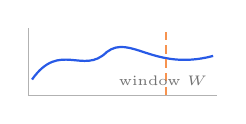
\begin{tikzpicture}
      \draw[black!30, line width=0.3pt] (0,0)--(2.4,0);
      \draw[black!30, line width=0.3pt] (0,0)--(0,0.85);
      \draw[primaryblue, line width=0.8pt]
        (0.05,0.2) .. controls (0.4,0.7) and (0.7,0.25) .. (1.0,0.55)
        .. controls (1.3,0.78) and (1.6,0.3) .. (2.35,0.5);
      \draw[accorange!80, line width=0.5pt, densely dashed] (1.75,0)--(1.75,0.85);
      \node[tiny@, text=black!55, anchor=south east] at (2.4,0.0) {window $W$};
    \end{tikzpicture}};
  \node[graysub, anchor=north, text width=3.0cm] at ([yshift=-2.5mm]m3c.south) {
    \textbullet~Accuracy\\[1pt]\textbullet~DP \quad \textbullet~EO\\[1pt]\textbullet~Loss};

% ---- 4 ADWIN Drift Detector -------------------------------------------
\modcard{m4}{16.6}{7.8}{3.7}{3.5}{orangemod}{accorange}{4.~ADWIN Detector}
  \node[orangesub, anchor=north, inner sep=2pt] at ([yshift=-7.0mm]m4.north) {
    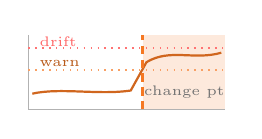
\begin{tikzpicture}
      \fill[accorange!16] (1.45,0) rectangle (2.5,0.95);
      \draw[black!30, line width=0.3pt] (0,0)--(2.5,0);
      \draw[black!30, line width=0.3pt] (0,0)--(0,0.95);
      \draw[accorange!85!black, line width=0.8pt]
        (0.05,0.2) .. controls (0.4,0.28) and (0.9,0.18) .. (1.3,0.24)
        -- (1.5,0.6) .. controls (1.8,0.78) and (2.1,0.62) .. (2.45,0.72);
      \draw[accorange, line width=0.8pt, densely dashed] (1.45,0)--(1.45,0.95);
      \draw[red!55, line width=0.5pt, dotted] (0,0.78)--(2.5,0.78);
      \draw[accorange!70, line width=0.5pt, dotted] (0,0.5)--(2.5,0.5);
      \node[tiny@, text=red!60, anchor=west]      at (0.02,0.86) {drift};
      \node[tiny@, text=accorange!75!black, anchor=west] at (0.02,0.58) {warn};
      \node[tiny@, text=black!55, anchor=south] at (1.98,0.02) {change pt};
    \end{tikzpicture}};
  \node[tiny@, text=black!55, anchor=south, align=center, text width=3.4cm] 
       at ([yshift=2.5mm]m4.south) {Hoeffding bound on rolling error};

% ---- 5 Reaction Controller --------------------------------------------
\modcard{m5}{21.1}{7.05}{4.1}{5.0}{orangemod}{accorange}{5.~Reaction Controller}
  % Each phase box: icon in a fixed left gutter aligned with the header row;
  % header and bullets share the same 5mm gutter indent for symmetric margins.
  \node[warnsub, anchor=north, text width=3.5cm] (r1) at ([yshift=-6.2mm]m5.north) {
    \hspace*{5mm}\textbf{\textcolor{accorange!80!black}{Warning}}\\[2pt]
    \hspace*{5mm}\textbullet~pre-warm LR\\[0pt]
    \hspace*{5mm}\textbullet~arm detectors};
  \path ([xshift=2.7mm,yshift=-3.4mm]r1.north west) pic[scale=0.44]{warning};

  \node[confsub, anchor=north, text width=3.5cm] (r2) at ([yshift=-2.5mm]r1.south) {
    \hspace*{5mm}\textbf{\textcolor{red!70!black}{Confirmed Drift}}\\[2pt]
    \hspace*{5mm}\textbullet~spike LR $\beta_c\eta_0$\\[0pt]
    \hspace*{5mm}\textbullet~sharpen $\tau\!\to\!\tau_{\mathrm{drift}}$\\[0pt]
    \hspace*{5mm}\textbullet~reset detectors};
  \fill[red!70!black] ([xshift=2.9mm,yshift=-3.6mm]r2.north west) circle (0.055);

  \node[recovsub, anchor=north, text width=3.5cm] (r3) at ([yshift=-2.5mm]r2.south) {
    \hspace*{5mm}\textbf{\textcolor{accgreen!70!black}{Recovery}}\\[2pt]
    \hspace*{5mm}\textbullet~anneal LR $\to\eta_0$\\[0pt]
    \hspace*{5mm}\textbullet~anneal $\tau\!\to\!1$};
  \path ([xshift=2.9mm,yshift=-3.6mm]r3.north west) pic[scale=0.42]{gear};

% ---- 7 Fairness Monitor -----------------------------------------------
\modcard{m7}{7.0}{2.4}{4.3}{3.9}{greenmod}{accgreen}{7.~Fairness Monitor}
  % corner icon: identical top-right offset as module 6 for consistent margins
  \path ([xshift=-3.6mm,yshift=-4.0mm]m7.north east) pic[scale=0.52]{scale};
  \node[greensub, anchor=north, inner sep=2pt] (m7c) at ([yshift=-7.5mm]m7.north) {
    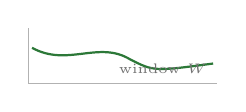
\begin{tikzpicture}
      \draw[black!30, line width=0.3pt] (0,0)--(2.4,0);
      \draw[black!30, line width=0.3pt] (0,0)--(0,0.7);
      \draw[accgreen!80!black, line width=0.8pt]
        (0.05,0.45) .. controls (0.5,0.2) and (0.9,0.55) .. (1.3,0.3)
        .. controls (1.6,0.15) .. (2.35,0.25);
      \node[tiny@, text=black!55, anchor=south east] at (2.4,0.0) {window $W$};
    \end{tikzpicture}};
  \node[graysub, anchor=north, text width=3.2cm] at ([yshift=-2.5mm]m7c.south) {
    \textbullet~Demographic Parity\\[1pt]\textbullet~Equalized Odds\\[1pt]\textbullet~Equal Opportunity};

% ---- 6 Training Update ------------------------------------------------
\modcard{m6}{12.0}{2.4}{4.3}{3.9}{greenmod}{accgreen}{6.~Training Update}
  % corner icon: identical top-right offset as module 7 for consistent margins
  \path ([xshift=-3.6mm,yshift=-4.0mm]m6.north east) pic[scale=0.55]{gear};
  \node[greensub, anchor=north, text width=3.5cm] (t1) at ([yshift=-7.0mm]m6.north) {
    sample $(x_t,y_t,a_t)$};
  \node[bluesub, anchor=north, text width=3.5cm, align=center] (t2) at ([yshift=-2.0mm]t1.south) {
    $\displaystyle \mathcal{L}=\mathcal{L}_{\mathrm{CE}}+\lambda\,\mathcal{L}_{\mathrm{fair}}$};
  \node[graysub, anchor=north, text width=3.5cm] (t3) at ([yshift=-2.0mm]t2.south) {
    \textbullet~node fairness penalty\\[1pt]\textbullet~gradient step (Adam) at $\eta_t$};

% =====================================================================
%  ARROWS  (blue solid = data ; orange dashed = drift/control)
% =====================================================================
% --- data-flow spine ---
\draw[dataflow] (m1.east) -- (m2.west) node[flowlbl,midway]{sample};
\draw[dataflow] (m2.east) -- (m3.west) node[flowlbl,midway]{prediction};
\draw[dataflow] (m3.east) -- (m4.west) node[flowlbl,midway]{errors};
% --- control flow inside the adaptation subsystem ---
\draw[ctrlflow] (m4.east) -- (m5.west) node[flowlbl,midway]{drift};

% controller -> training update (control), routed through the open lower-right
\draw[ctrlflow] (m5.south west) .. controls (17.0,4.0) and (14.5,3.7) .. (m6.east)
  node[flowlbl,pos=0.32]{LR\,$\eta_t$};

% controller -> forest (control: reset trees / anneal temperature)
\draw[ctrlflow] (m5.north) .. controls ($(m5.north)+(0,1.25)$) and ($(m2.north)+(0,1.25)$) ..
  (m2.north) node[flowlbl,pos=0.5]{reset trees / anneal $\tau$};

% --- feedback loop : Training Update -> Fair Oblique Forest ---
\draw[dataflow] (m6.north) .. controls +(0,1.0) and +(1.6,-1.0) .. ([xshift=10mm]m2.south)
  node[flowlbl,pos=0.5]{updated forest parameters};

% forest -> fairness monitor (node statistics)
\draw[dataflow] (m2.south west) .. controls +(-0.3,-1.1) and +(-0.3,1.1) .. (m7.north west)
  node[flowlbl,pos=0.5,xshift=-3mm]{node-level stats};

% fairness monitor -> training update (fairness penalty)
\draw[dataflow] (m7.east) -- (m6.west) node[flowlbl,midway,align=center]{fairness\\penalty};

% =====================================================================
%  CONTAINER LABELS
% =====================================================================
\node[font=\footnotesize\bfseries, text=primaryblue!80, anchor=south west]
  at (-0.4,10.2) {Main learning pipeline};
\node[font=\footnotesize\bfseries, text=accorange!85!black, anchor=south east]
  at (23.2,10.2) {Adaptation subsystem};

% =====================================================================
%  LEGEND  (occupies the freed lower-right area)
% =====================================================================
\node[rounded corners=4pt, draw=black!30, fill=white, line width=0.6pt,
      inner sep=6pt, anchor=south east, align=left,
      blur shadow={shadow blur steps=6, shadow yshift=-0.8pt, shadow opacity=16}]
      (leg) at (23.3,0.7) {
  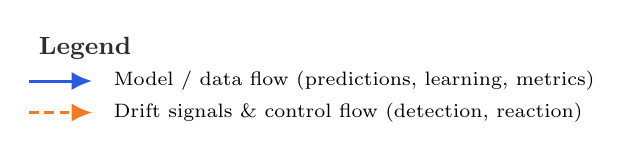
\begin{tikzpicture}[baseline]
    \node[font=\small\bfseries, anchor=west, text=darktext] at (0,0.6) {Legend};
    \draw[dataflow] (0,0.18)--(0.8,0.18);
    \node[body, anchor=west] at (0.95,0.18) {Model / data flow (predictions, learning, metrics)};
    \draw[ctrlflow] (0,-0.22)--(0.8,-0.22);
    \node[body, anchor=west] at (0.95,-0.22) {Drift signals \&\ control flow (detection, reaction)};
  \end{tikzpicture}};

\end{tikzpicture}
\end{document}